\section{Method Overview}
\label{sec:overview}

In this section, we carefully analyze existing agent memory systems across the four components in Section~\ref{sec:def} and establish a unified taxonomy that summarizes representative component methods.

% \zw{module figures to be added!}
% \zw{emphasize the difference between memory representation and memory indexing and storage, memory extraction}

\subsection{Memory Representation and Storage}
\label{subsec:represent}

\begin{figure}[!t]
  \centering
  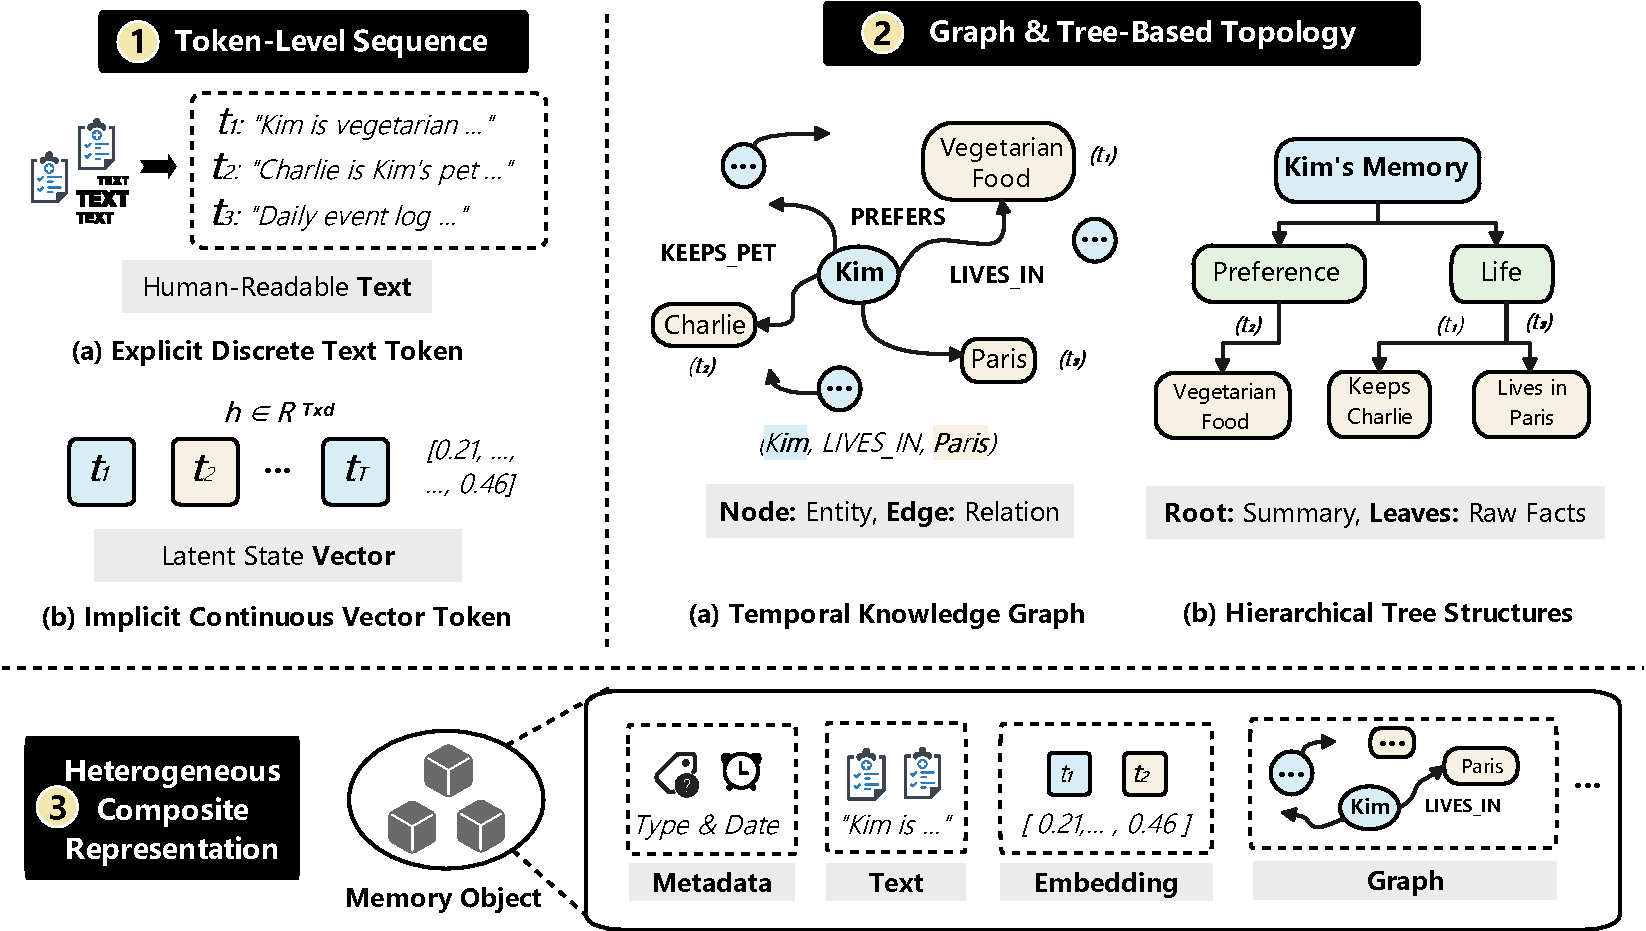
\includegraphics[width=\linewidth]{figures/memory_representation_v3.pdf}
  \vspace{-.5cm}
  \caption{Memory Representation Methods.}
  \label{fig:memory_representation}
  \vspace{-.5cm}
\end{figure}

% \zw{data model}

% \zw{continuous hidden vectors or standard discrete token sequences}

This module consists of two components:
(1) logical representation, which defines the structural encoding and organization exposed to the agent system, directly dictating capacity, accessibility, and trade-offs in expressiveness, retrieval granularity, and downstream reasoning compatibility;
and (2) physical storage, which designates the persistence and indexing structures, such as volatile in-context registers, dense vector engines, or topological graph databases.

% A suitable representation can improve how agents preserve long-term context, connect related facts, and reuse past experience, while an unsuitable one may limit retrieval precision, increase storage overhead, or make memory updates difficult. 
% \zw{discuss advantages and disadvantages of each representation (characteristics)}

\subsubsection{\textbf{Logical Representation}}
As displayed in Figure~\ref{fig:memory_representation}, this component acts as a bridge between raw data and the execution environment by organizing memory into clear models, such as graphs, or vector spaces.
It determines how efficiently a system can search, combine, and use historical context for complex tasks.

\noindent \ding{182} \textbf{Token-Level Sequence Representation.} This category models memory as flat, one-dimensional sequences lacking explicit structural abstractions (e.g., graphs or hierarchies). Memory is represented either as discrete, human-readable natural language tokens or as implicit, continuous latent vector tokens (e.g., fact embeddings, hidden states, or KV-cache tensors).

\noindent \underline{\textit{$\blacktriangleright$ Explicit Discrete Text Token.}}
This category models memory as human-readable strings or independent factual statements.
For instance, Mem0 isolates memory into discrete natural language facts extracted directly from interaction history. Similarly, MemoChat structures multi-turn dialogues into discrete JSON blocks (topics, summaries, raw turns) to maintain topical coherence within a plain-text paradigm. While these systems externalize their plain-text memory, others retain it within the active processing window: MemAgent restricts its internal belief state to a strictly bounded text sequence (e.g., 1024 tokens), and MEM1 encapsulates internal-state summaries within specialized boundary tags (e.g., <IS>).

\begin{sloppypar}
\noindent \underline{\textit{$\blacktriangleright$ Implicit Continuous Vector Token.}}
Departing from readable text tokens, this sub-category encodes memory as continuous vectors, which may be materialized either as external embeddings attached to facts and summaries for semantic retrieval, or as model-side latent states such as compressed internal states and attention caches.
For example, Mem0 represents extracted facts as dense semantic embeddings and MemoRAG utilizes specifically initialized weight matrices to compress raw inputs into high-dimensional Key-Value (KV) cache tensors. 
Although these vector-token representations reduce explicit tokenization burdens and integrate naturally with retrieval or inference pipelines, they sacrifice structural interpretability and are difficult to manipulate via fine-grained operations, such as predicate-level filtering or targeted updates to encoded facts.
% Although these continuous tokenization methods reduce explicit storage burdens and integrate with inference pipelines, they sacrifice structural interpretability and pose challenges for conventional data management operations (e.g., SQL-based filtering).
\end{sloppypar}

% \zw{1. end-to-end optimization; 2. fix length; all incorporate RL mechanism?}

\noindent \ding{183} \textbf{Graph and Tree-Based Topological Representation.}
This category abstracts memory into structured graph and tree topologies with interconnected nodes and edges, allowing conversational entities, high-level concepts, and their temporal or semantic relationships to be explicitly modeled and computationally traversed.

\begin{figure}[!t]
  \centering
  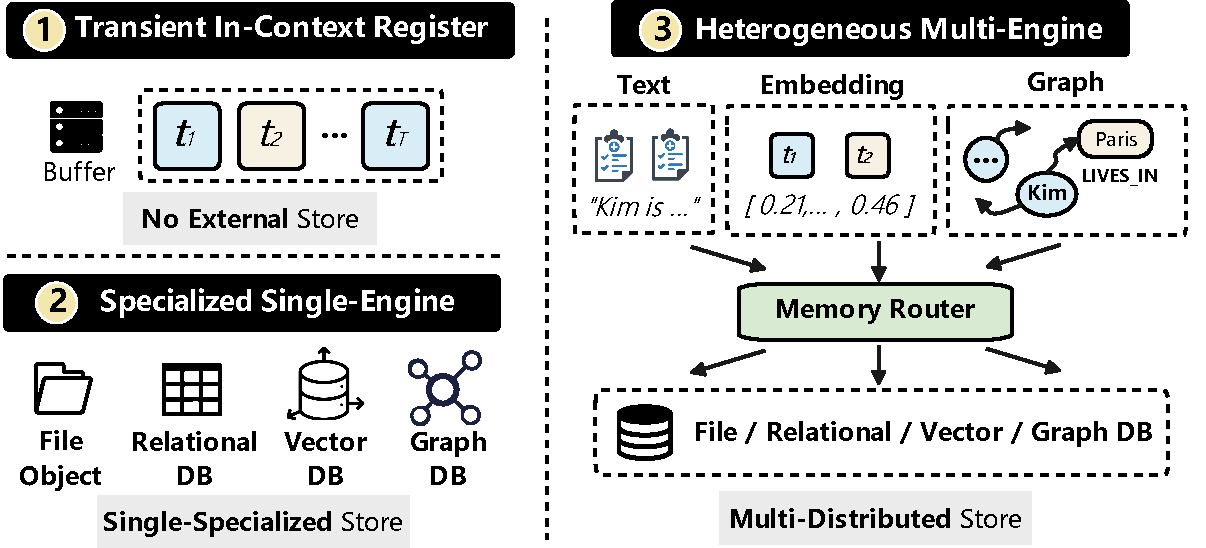
\includegraphics[width=\linewidth]{figures/memory_storage_v3.pdf}
  % \vspace{-.75cm}
  \caption{Memory Storage Methods.}
  \label{fig:memory_storage}
  \vspace{-.75cm}
\end{figure}

% for computational traversal.


\noindent \underline{\textit{$\blacktriangleright$ Temporal Knowledge Graphs.}}This sub-category models memory using graph topologies to map entities and their interconnections, natively supporting temporal reasoning and conflict detection.
For example, Zep partitions memory into formally defined, temporally-aware knowledge graphs (e.g., episode, entity, and community subgraphs). Similarly, $\text{Mem0}^g$ formalizes memory as a directed labeled graph, where vertices represent entities and edges encapsulate relationship triplets (e.g., ``LIVES\_IN''). To aid temporal reasoning, entity nodes are enriched with structural metadata like semantic types, dense embeddings, and creation timestamps.

\noindent \underline{\textit{$\blacktriangleright$ Hierarchical Tree Structures.}}
This sub-category organizes knowledge into recursive, hierarchical structures, preserving highly granular observations at terminal leaves and broad semantic abstractions at ancestor nodes. For example, MemTree models memory as a dynamic, directed tree schema. Each node is structured as a tuple containing textual content, a dense embedding, topological pointers, and a depth scalar. Within this topology, deep leaf nodes retain isolated facts (e.g., a player scoring), while ancestor nodes provide high-level conceptual summaries (e.g., the match result), with a specialized root node serving as the definitive entry point.
% for retrieval traversals.

% These methods provide stronger structural organization than plain-text memory and are well suited for relation-aware reasoning, multi-hop retrieval, and long-range knowledge integration.

% GraphRAG constructs a knowledge graph with entities as nodes, weighted relations as edges, and claims as attached properties. HippoRAG and HippoRAG 2 represent noun phrases and paragraphs as nodes, augmented with knowledge graph triples and dense vector embeddings. 

\noindent \ding{184} \textbf{Heterogeneous Composite Representation.}
This category moves past simple token sequences and standard graphs by packaging memory into complex, multi-part data containers. These architectures directly combine unstructured text with highly structured metadata (e.g., timestamps, categorical labels, vector embeddings, and network links) to form a single functional unit. For example, MemOS proposes the MemCube, a unified data object that organizes memory into three distinct payloads (plain-text, activation, and parametric memory) alongside structured details (e.g., ID tags).
% like descriptive ID tags. 

% Similarly, A-MEM models its basic unit as highly modular, interconnected knowledge records (i.e., Zettelkasten-inspired atomic notes). In this system, each individual unit holds the original raw content along with temporal bounds, dense vector representations, and explicit adjacency links to other notes.

% Expanding on this partitioning strategy, MIRIX separates memory into six structurally different textual schemas (including core, episodic, semantic, procedural, and resource memory) to isolate distinct functional tasks.

% Ultimately, these composite methods (e.g., variants also utilized by SimpleMem and EverMemOS) offer a balanced logical design: they preserve the semantic richness of raw text while enabling explicit programmatic control, exact database indexing, and rigorous data management.

\subsubsection{\textbf{Physical Storage and Indexing}}
As shown in Figure~\ref{fig:memory_storage}, this component manages how data is physically stored and accessed, relying on systems like in-memory caches, files, vector engines, or databases.
It sets the actual capacity limits and determines the speed, throughput, and overall scalability of memory operations.

\noindent \ding{182} \textbf{Transient In-Context Register.}
To eliminate disk I/O and external traversal latency, this category retains memory exclusively within the active hardware state (e.g., dynamic context windows or KV caches).
MemoChat avoids dedicated external memory engines and keeps structured JSON-style memos within the LLM context input during its memorization-retrieval-response loop, while MemAgent directly stores summary tokens as Key-Value (KV) cache tensors via dense positional embeddings.
% while MemAgent opts for an in-context volatile mechanism where summary tokens reside directly as Key-Value (KV) cache tensors via dense positional embeddings.

\begin{figure}[!t]
    % \vspace{-1.cm}
  \centering
  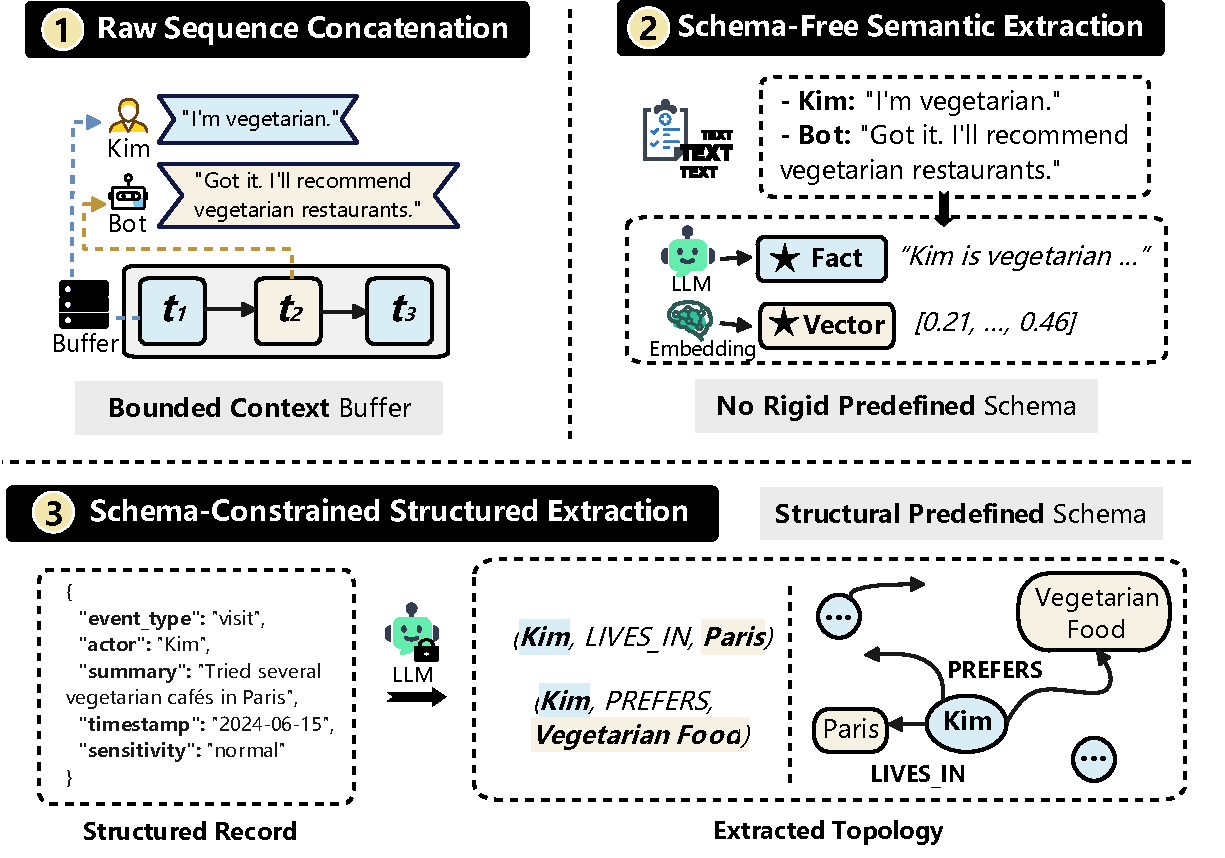
\includegraphics[width=\linewidth]{figures/memory_extraction_v2.pdf}
  \vspace{-.75cm}
  \caption{Memory Extraction Methods.}
  \label{fig:memory_extraction}
  \vspace{-.3cm}
\end{figure}


\noindent \ding{183} \textbf{Specialized Single-Engine Storage.}
This category physically warehouses formulated units within a standalone, homogeneous backend strictly tailored to the memory's logical structure.
Depending on the ingestion paradigm, architectures deploy specific backend topologies: 
(1) \textit{Dense Vector Databases} are utilized to project data into continuous high-dimensional spaces; Mem0 and MemTree use centralized vector stores, Letta leverages PostgreSQL with the \texttt{pgvector} extension;
(2) \textit{Graph Databases} are deployed to enforce topological constraints; both Zep and $\text{Mem0}^g$ execute predefined Cypher queries to physically persist logical graph components into Neo4j;
(3) \textit{Relational SQL Engines} are used to serialize structural and temporal schemas.
LightMem incrementally appends factual streams to preserve global relational states;
(4) \textit{File or Object Stores} preserve raw interaction artifacts (e.g., conversation histories or tool-execution logs) as files or object blobs.

% MIRIX persistently commits its abstractions to a lightweight \texttt{sqlite.db} file to reduce storage footprints

\noindent \ding{184} \textbf{Heterogeneous Multi-Engine Storage.}
This category dynamically constructs multiple index typologies or distributes data across heterogeneous backends (e.g., pairing a dense vector store with a topological graph database). SimpleMem ingests memory into LanceDB with an IVF-PQ mechanism that concurrently maintains dense embeddings, sparse BM25 indices, and SQL predicates. MemoryOS relies on a hybrid index fusing dense cosine similarity with discrete Jaccard similarity. Conversely, MemOS delegates serialized payloads to highly specialized independent backends, fusing Vector and Graph databases via a standardized memory adapter interface.

% EverMemOS pairs dense vector representations alongside exact-match sparse representations.

\subsection{Memory Extraction}
\label{subsec:storage}

Memory extraction concerns how raw interaction traces are computationally processed.
It covers both the extraction pipeline, how language models extract, summarize, or parse unstructured text into logical structures.
As shown in Figure~\ref{fig:memory_extraction}, it defines how the agent memory system transforms heterogeneous input streams (e.g., multi-turn dialogues, and tool execution logs) into logical memory primitives prior to physical persistence.

\noindent \ding{182} \textbf{Raw Sequence Concatenation.}
To minimize computational overhead, this category bypasses explicit extraction prompts, formulating memory directly as raw token concatenations or transient state summaries (e.g., appending recent dialogue turns directly into a prompt buffer).
Systems such as MEM1 and MemAgent retain their newly formulated structures exclusively within the active computational state without secondary parsing.

\noindent \ding{183} \textbf{Schema-Free Semantic Extraction.}
This category systematically distills raw, unstructured inputs into independent, high-value informational units, representing them either as explicit free-form texts or as compressed, continuous latent vectors.
By isolating core knowledge from broader conversational context, it ensures precise and granular retrieval.
For example, Mem0  actively parses interactions to extract and store discrete, standalone factual statements (e.g., ``User is vegetarian and dairy-free'').
% MemoryBank distills raw dialogue logs into condensed daily event narratives and free-text personality descriptors (e.g., ``introverted, determined, ambitious'').
% Conversely, MemoRAG departs from symbolic text generation entirely, using dedicated weight matrices to mathematically compress raw input sequences into continuous latent KV-cache tensors.

\begin{figure}[!t]
    % \vspace{-.5cm}
  \centering
  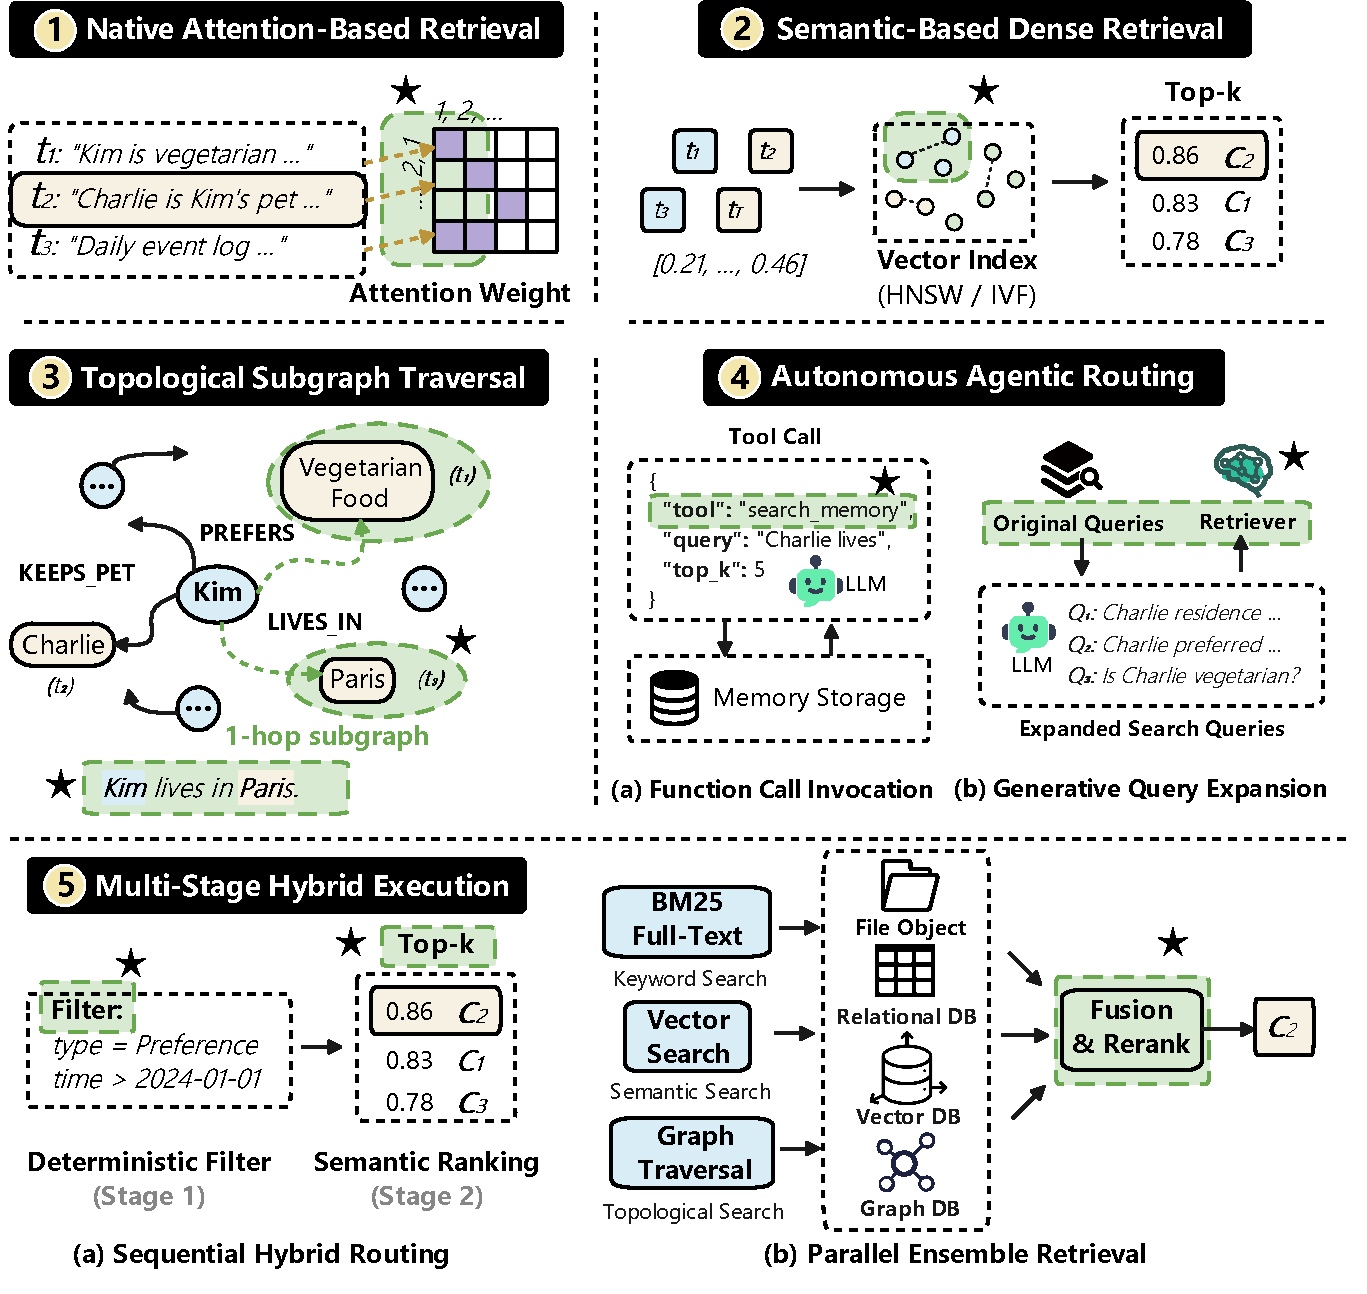
\includegraphics[width=\linewidth]{figures/memory_retrieval_v3.pdf}
  \vspace{-.75cm}
  \caption{Memory Retrieval Methods.}
  \label{fig:memory_retrieval}
  \vspace{-.65cm}
\end{figure}


\noindent \ding{184} \textbf{Schema-Constrained Structured Extraction.}
This category prompts the LLM to parse raw inputs and synchronously populate a rigidly predefined structural schema, producing strictly typed data rather than free-form text. The constrained output takes the form of either topological entity-relation triplets for graph insertion or multi-modal relational payloads for hybrid storage, depending on the target backend.
Zep and $\text{Mem0}^g$ extract typed directed relational edges (e.g., \texttt{LIVES\_IN}, \texttt{WORKS\_AT}) conforming to predefined graph schemas, with Zep additionally applying a reflection-inspired verification step to suppress hallucinated triplets.
MemoChat populates predefined structural fields to ensure data predictability by leveraging \llms to segment conversations into strict JSON schemas.
% SimpleMem concurrently produces dense embeddings, sparse BM25 vectors, and standardized ISO-8601-normalized metadata from a single interaction unit.

% MIRIX populates predefined relational table fields including event type, actor, summary, and timestamp alongside sensitivity-level metadata.

% EverMemOS simultaneously populates four typed MemCell fields: a narrative episode, atomic facts, a temporal foresight interval, and originating source metadata.

\subsection{Memory Retrieval and Query Routing}
\label{subsec:retrieval}

Memory retrieval and query routing determine how the agent memory system dynamically identifies and extracts relevant historical context to inform the overarching agent's current reasoning state.
As shown in Figure~\ref{fig:memory_retrieval}, this module encompasses the complete query execution spectrum, defining the operational algorithms, predicate evaluations, and agentic workflows utilized to traverse indices. 

% In agent memory systems, retrieval is often more than simple lookup, as it may require structured navigation, adaptive tool use, intermediate planning, or post-retrieval evidence aggregation.
% These strategies range from implicit self-attention scans within volatile memory, to explicit metric searches over external databases, and ultimately to complex, multi-stage hybrid pipelines orchestrating autonomous retrieval.


\noindent \ding{182} \textbf{Native Attention-Based Retrieval.}
To bypass external database I/O, this category uses the transformer's native computational graph as the sole retrieval engine, relying entirely on self-attention mechanisms to implicitly weight and route information (e.g., scanning dialogue tokens directly within the KV cache). MEM1 performs implicit retrieval via self-attention over the current sequence, utilizing a two-dimensional attention mask to preserve causal consistency. MemAgent implements routing by concatenating blocks directly into the prompt template, enabling standard attention-based decoding without external cross-encoder reranking.

\noindent \ding{183} \textbf{Semantic-Based Dense Retrieval.}
Operating over continuous latent spaces, this category maps query tensors against uniform vector indices to extract localized spatial neighbors (e.g., executing a standard $K$-Nearest Neighbors (KNN) search). Mem0 calculates vector embeddings for incoming queries to execute a dense similarity search, fetching a constrained subset of facts. LightMem utilizes efficient cosine-similarity distance calculations over dense embeddings, bypassing computationally expensive iterative reranking. MemTree implements a collapsed-tree architecture that mathematically flattens its hierarchy, broadcasting inbound vectors to compute global cosine-similarity distributions across all candidates.

% Similarly, MemoryBank orchestrates a dense single-stage pipeline via FAISS to identify nearest neighbors before structuring the outputs into a meta-prompt.

\noindent \ding{184} \textbf{Topological Subgraph Traversal.}
Departing from continuous vector spaces, this category retrieves information by traversing explicit relationship edges to extract semantic clusters structurally grounded in knowledge graphs (e.g., hopping from a \texttt{User} node to a linked \texttt{Preference} node).
$\text{Mem0}^g$ deploys an entity-centric heuristic to recursively traverse local subgraphs synchronously with semantic triplet evaluations.
A-MEM identifies candidate anchors via dense $K$-Nearest Neighbor selection, then executes localized graph traversal to access topologically adjacent memory nodes explicitly linked within the same conceptual cluster.

\noindent \ding{185} \textbf{Autonomous Agentic Routing.}
Rather than executing deterministic database scans, this category delegates retrieval to the \llm itself, thereby functioning as an active, autonomous query planner. It generates tool-call invocations or drafts implicit search criteria.
% prior to executing the database scan.

\begin{sloppypar}
\noindent \underline{\textit{$\blacktriangleright$ \textbf{Function Call Invocation}.}}
This sub-category bridges the \llm with external storage by generating explicit function call commands to directly execute predefined database operations (e.g., outputting a valid JSON payload to trigger an external database API). For example, Letta orchestrates self-directed memory retrieval where the LLM evaluates its active context to explicitly generate localized function calls (e.g., emitting an \texttt{archival\_storage.search()} command to extract targeted historical logs).
\end{sloppypar}

\begin{sloppypar}
\noindent \underline{\textit{$\blacktriangleright$ \textbf{Generative Query Expansion}.}}
Unlike rigid function calling, this approach uses natural language generation to synthesize intermediate clues or decompose complex intents before mapping them to the index (e.g., rewriting vague prompts into descriptive search strings). SimpleMem uses an Intent-Aware Retrieval Planning module where the \llm dissects queries, calculates adaptive search depths, and synthesizes optimized query variants.
\end{sloppypar}

% MemoRAG employs a two-stage paradigm where a latent memory model generates a draft textual answer, which then serves as a high-semantic search clue routed to an external dense retriever.

\begin{figure}[!t]
  \centering
  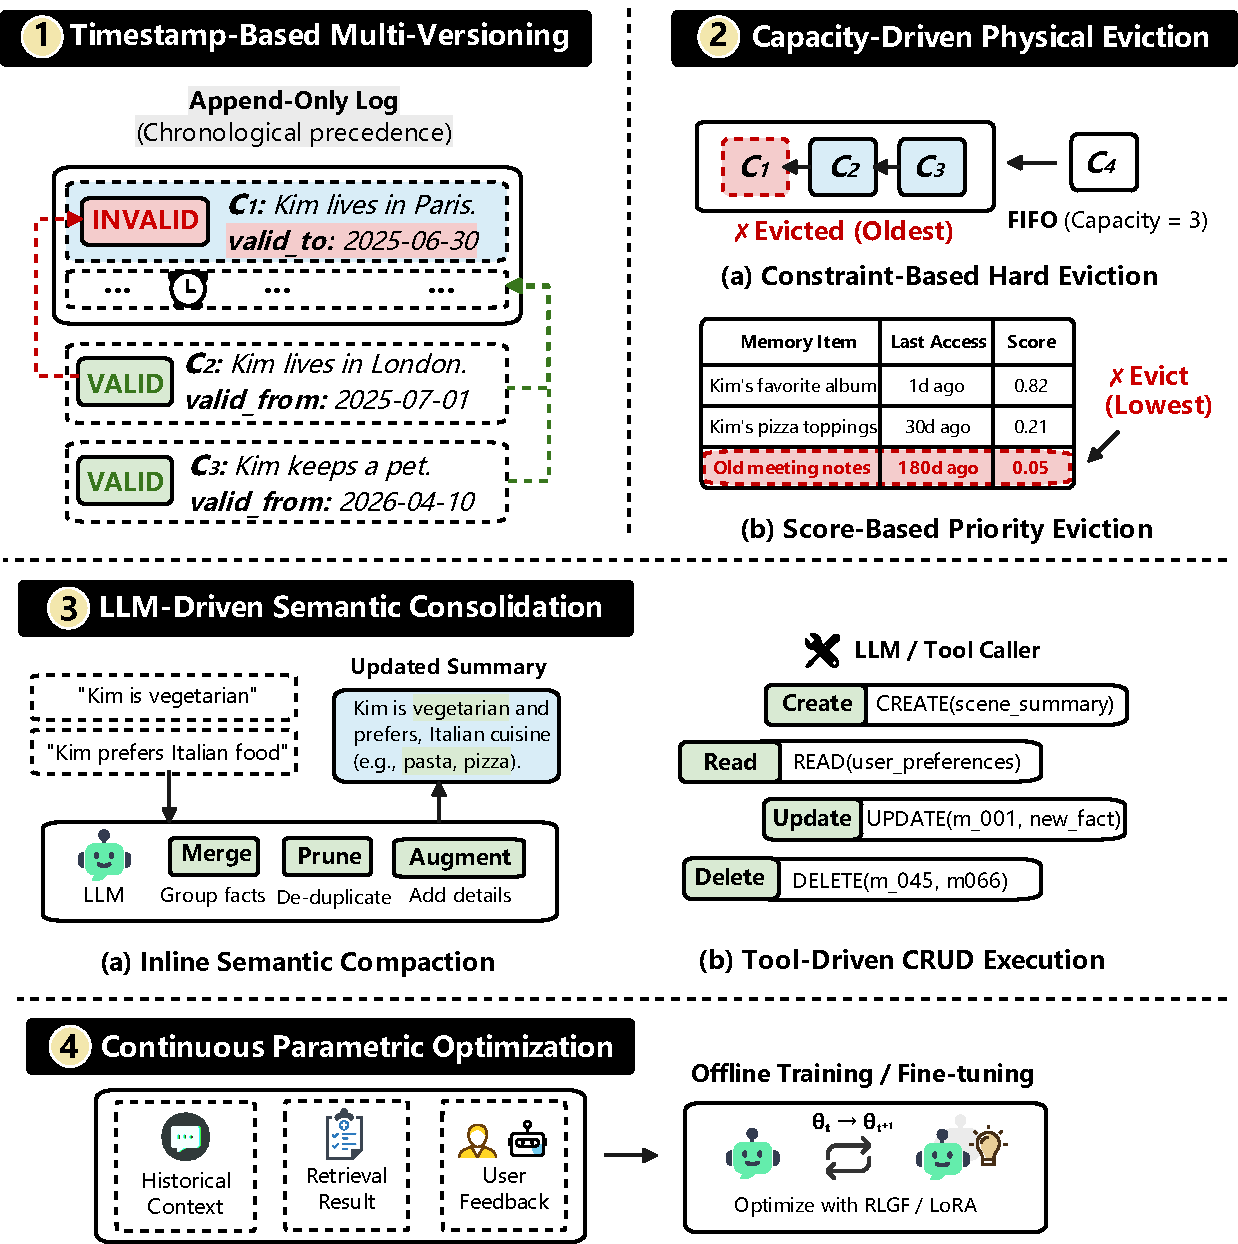
\includegraphics[width=\linewidth]{figures/memory_maintenance_v2.pdf}
  \vspace{-.5cm}
  \caption{Memory Maintenance Methods.}
  \label{fig:memory_maintenance}
  \vspace{-.65cm}
\end{figure}


\noindent \ding{186} \textbf{Multi-Stage Hybrid Execution.}
To overcome the recall limitations of single-paradigm searches, this category executes multi-engine query pipelines orchestrating multi-dimensional candidate generation followed by downstream reranking frameworks.

\noindent \underline{\textit{$\blacktriangleright$ \textbf{Sequential Hybrid Routing}.}}
This sub-category chains retrieval paradigms into a strictly ordered pipeline, systematically pruning the search space with deterministic predicates before executing fine-grained semantic extraction (e.g., applying strict SQL date filters before computationally expensive vector searches). MemoryOS executes a federated routing strategy featuring coarse-grained predicate evaluation followed by fine-grained semantic ranking strictly within isolated segments.
It algebraically fuses rule-based structural Boolean filtering with dense semantic similarity routing.

\noindent \underline{\textit{$\blacktriangleright$ \textbf{Parallel Ensemble Retrieval}.}}
In contrast to sequential filtering, this approach maximizes initial recall by simultaneously dispatching queries to multiple distinct indexing algorithms, followed by a late-stage fusion and reranking phase to optimize the aggregated pool (e.g., concurrently fetching candidates via BM25 and dense vector search, then cross-encoding the results). Zep executes simultaneous cosine semantic scans, Okapi BM25 full-text searches, and topological BFS, subsequently optimizing precision via RRF, MMR, and computationally intensive cross-encoder models. 

% MIRIX invokes an LLM compiler to generate a synthesized target topic, then algorithmically routes the query through a hybrid suite of dense, sparse, and exact-string-match algorithms.

% EverMemOS fuses dense and sparse scores through an RRF algorithm, executes a Qwen3-Reranker phase supported by temporal logical predicate pushdowns, and concludes with an LLM-based verification.

\subsection{Memory Maintenance}
\label{subsec:maintenance}

Memory maintenance concerns how memory is updated, maintained, compressed, forgotten, and eventually removed over time.
As shown in Figure~\ref{fig:memory_maintenance}, it captures the dynamic behavior of memory after it has been created, including how new information is incorporated, how outdated or conflicting content is revised, and how the system controls memory growth under limited resources.
% It directly affects the long-term quality, consistency, and efficiency of agent memory.
% In practice, lifecycle management determines whether memory remains useful and coherent as the agent continues to learn from evolving interactions and environments.

\begin{figure*}[!t]
\vspace{-.5cm}
\centering
\vspace{-.75cm}
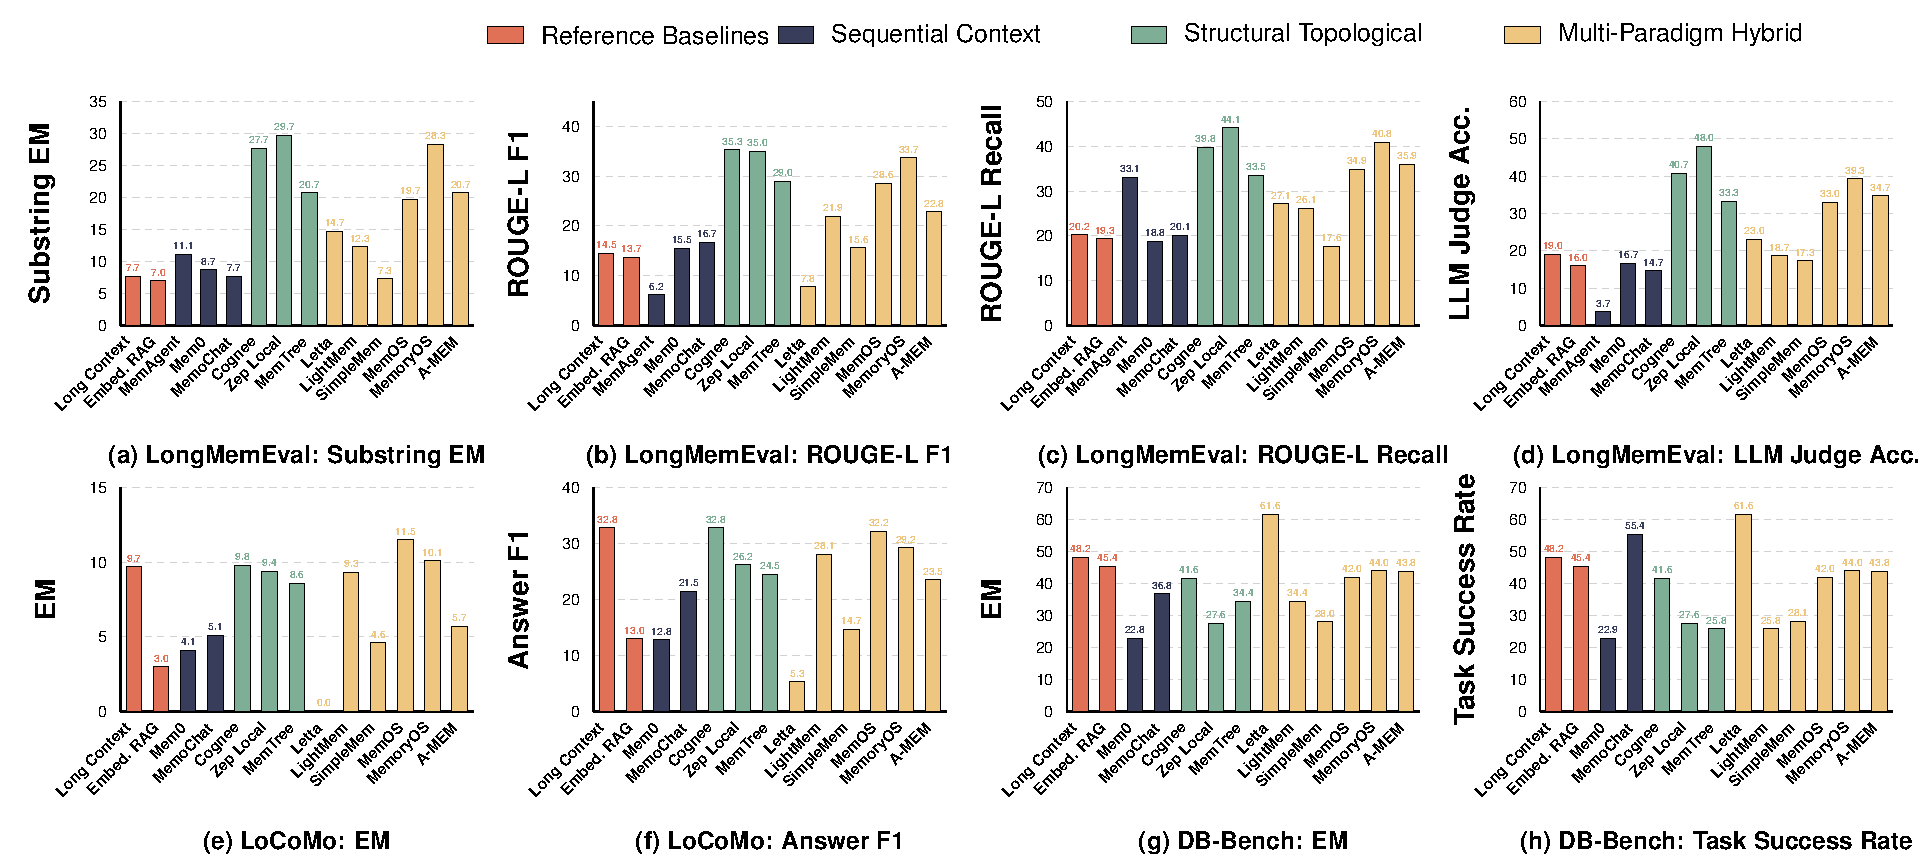
\includegraphics[width=\linewidth]{figures/table2_barchart_v2.pdf}
\caption{Effectiveness of Memory Systems over \textit{LoCoMo}, \textit{MemoryAgentBench (LongMemEval)}, \textit{LifeLongAgentBench (DB-Bench)}.}
\vspace{-.5cm}
\label{fig:RQ1_effectiveness}
\end{figure*}

\noindent \ding{182} \textbf{Timestamp-Based Multi-Versioning.}
Rather than executing physical row deletions, this category preserves historical continuity by utilizing timestamp metadata and append-only logs to logically deprecate expired facts.
Operating via explicit metadata mutations, Zep and $\text{Mem0}^g$ avoid physical deletion by marking obsolete or conflicting relationships as logically invalid using validity flags and timestamps.
Taking an append-only approach, LightMem incrementally inserts timestamped factual streams, while SimpleMem resolves contradictions through strict chronological precedence using ISO-8601 timestamps.
Synthesizing these techniques, MemOS leverages a structured Update API to execute differential writes, seamlessly updating provenance IDs to generate multi-version chains.

\noindent \ding{183} \textbf{Capacity-Driven Physical Eviction.}
In contrast to timestamp-based multi-versioning, this category manages unbounded memory growth by physically dropping or unconditionally overwriting data.
It executes this physical pruning through either strict deterministic constraints or dynamically calculated eviction scores.

\noindent \underline{\textit{$\blacktriangleright$ \textbf{Constraint-Based Hard Eviction}.}}
This sub-category enforces rigid execution bounds by utilizing deterministic rules—such as strict FIFO queues, fixed sequence boundaries, or hard token limits—to unconditionally evict older states.
Executing structural overwrites, MemAgent implements a programmatic scheduling algorithm that unconditionally replaces older memory sequences with newly synthesized summary blocks at every fixed segment boundary. Enforcing hard capacity limits, MEM1 operates through a system-enforced truncation mechanism that executes an automated FIFO pruning protocol to evict older tags once active context thresholds are breached. Operating via threshold flushes, Letta strictly handles buffer capacities via an OS-inspired queue manager; when the token count breaches a terminal limit, it forces a flush sequence to evict older messages into secondary recall storage.

\noindent \underline{\textit{$\blacktriangleright$ \textbf{Score-Based Priority Eviction}.}}
Rather than relying on static capacity limits, this sub-category dynamically forces the physical obsolescence of data by continuously calculating temporal decay or access-frequency scores.
Quantifying access frequency, MemoryOS measures segment vitality via a scalar Heat score that balances retrieval frequency against exponential temporal decay, executing priority evictions that physically target the lowest-heat segments.

% Applying mathematical decay curves, MemoryBank governs state maintenance via an Ebbinghaus Forgetting Curve algorithm, aggressively decaying retention probability over elapsed time while systematically extending persistence by resetting decay variables for recently retrieved contexts.

% SELF-RAG evaluates valid states locally during the active decoding step via self-critique, handling contradiction deterministically by algorithmically pruning unsupported generation branches.

\noindent \ding{184} \textbf{\llm-Driven Semantic Consolidation.}
Operating as a cognitive governor, this category leverages the \llm to dynamically resolve logical conflicts and abstract redundant observations into dense summaries prior to query or persistence phases.

\begin{sloppypar}
\noindent \underline{\textit{$\blacktriangleright$ \textbf{Inline Semantic Compaction}.}}
During the active write phase, this sub-category dynamically evaluates and consolidates newly ingested data against existing memory nodes, systematically merging redundant assertions prior to database transaction commitment (e.g., compressing three similar dialogue turns into one dense summary node).
SimpleMem executes online semantic synthesis on-the-fly, systematically merging structurally similar assertions into singular dense abstractions prior to database transaction commitment. MemTree utilizes a core scheduling operation that recursively triggers a semantic summarization prompt across all parent nodes to dynamically fuse historical states with novel payloads.
\end{sloppypar}

% EverMemOS enforces recency-aware profile evolution, prompting the LLM to synthesize updated scene summaries that directly resolve logical conflicts. A-MEM evaluates surrounding networks via designated prompts to execute deterministic mutation actions such as ``strengthen'', ``merge'', or ``prune''.

\begin{sloppypar}
\noindent \underline{\textit{$\blacktriangleright$ \textbf{Tool-Driven CRUD Execution}.}}
In contrast to automated fusion, this sub-category operationalizes maintenance through discrete, programmed state-mutations guided explicitly by \llm-driven tool interfaces that issue explicit Create, Read, Update, or Delete (CRUD) commands. Mem0 operationalizes its dynamic maintenance strictly through structured \llm tool-calling interfaces encompassing discrete programmed state-mutations such as UPDATE, and DELETE.
\end{sloppypar}

% MIRIX orchestrates persistent state transitions via a decentralized multi-agent architecture where a central Meta Memory Manager routes semantic update commands to specialized peripheral domain managers.

\noindent \ding{185} \textbf{Continuous Parametric Optimization.}
Completely decoupling state updates from online inference latency, this category executes heavy neural optimizations as asynchronous background processes, modifying the actual model parameters rather than the external database schema (e.g., running continuous fine-tuning on overnight batches).
For example, MemoRAG leaves active inference tokens strictly static and read-only, optimizing extraction quality exclusively during an offline training phase via a Reinforcement Learning with Generation Feedback (RLGF) algorithmic framework. 

% MemoryBank performs continuous Parameter-Efficient Fine-Tuning using the Low-Rank Adaptation (LoRA) algorithm on accumulated historical dialogues to dynamically align the model's fundamental behavioral state.
% without requiring real-time database schema mutations.
